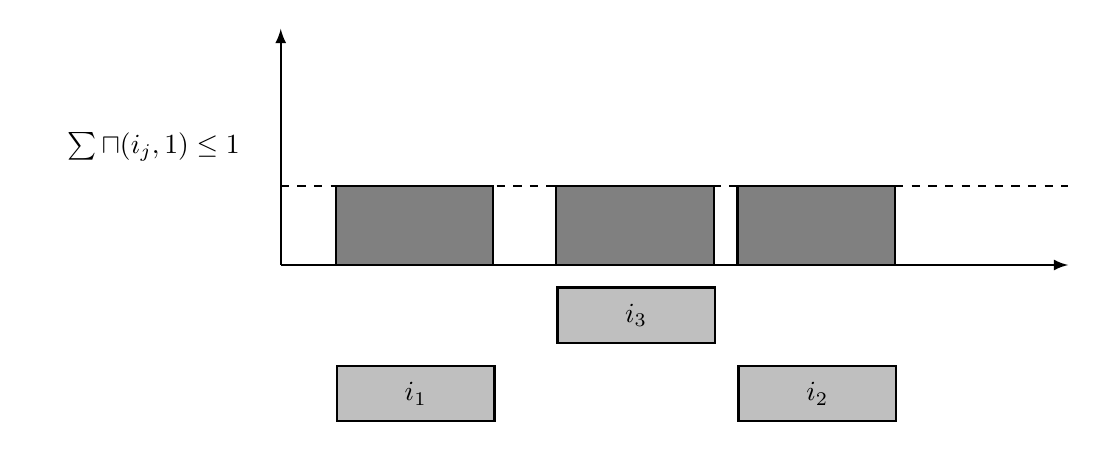
\begin{tikzpicture}
        \draw  (0.7,1) node[draw, thick, fill=lightgray, rectangle, anchor=south west, inner sep=0pt, minimum width=2cm, minimum height=0.7cm] {\textbf{$i_1$}};
        \draw  (5.8,1) node[draw, thick, fill=lightgray, rectangle, anchor=south west, inner sep=0pt, minimum width=2cm, minimum height=0.7cm] {\textbf{$i_2$}};
        \draw  (3.5,2) node[draw, thick, fill=lightgray, rectangle, anchor=south west, inner sep=0pt, minimum width=2cm, minimum height=0.7cm] {\textbf{$i_3$}};
        \draw[thick, -latex] (0,3) -- (0,6) node[midway, left, minimum width=3.2cm] {$\sum \sqcap(i_j, 1) \leq 1$};

        \draw[thick, fill=gray] (0.7,3) -- (0.7,4) -- (2.7,4) -- (2.7,3) -- (3.5,3) -- (3.5,4) -- (5.5,4) -- (5.5,3) -- (5.8,3) -- (5.8,4) -- (7.8,4) -- (7.8,3);
        \draw[thick, dashed] (0,4) -- (10,4);
        \draw[thick, -latex] (0,3) -- (10,3);
    \end{tikzpicture}
